\documentclass[a4paper,12pt]{article}

%%% Работа с русским языком
\usepackage{cmap}					% поиск в PDF
\usepackage{mathtext} 				% русские буквы в фомулах
\usepackage[T2A]{fontenc}			% кодировка
\usepackage[utf8]{inputenc}			% кодировка исходного текста
\usepackage[english,russian]{babel}	% локализация и переносы
\usepackage{geometry} % Меняем поля страницы
\geometry{left=2cm}% левое поле
\geometry{right=1.5cm}% правое поле
\geometry{top=1cm}% верхнее поле
\geometry{bottom=2cm}% нижнее поле

%%% Дополнительная работа с математикой
\usepackage{amsfonts,amssymb,amsthm,mathtools} % AMS
\usepackage{amsmath}
\usepackage{icomma} % "Умная" запятая: $0,2$ --- число, $0, 2$ --- перечисление
\usepackage{pdflscape}
\usepackage[dvipsnames]{xcolor}
\usepackage{diagbox}
\usepackage{tikz}
\usetikzlibrary{automata,positioning}
%% Номера формул
%\mathtoolsset{showonlyrefs=true} % Показывать номера только у тех формул, на которые есть \eqref{} в тексте.

%% Шрифты
\usepackage{euscript}	 % Шрифт Евклид
\usepackage{mathrsfs} % Красивый матшрифт

%% Свои команды
\DeclareMathOperator{\sgn}{\mathop{sgn}}

%% Перенос знаков в формулах (по Львовскому)
\newcommand*{\hm}[1]{#1\nobreak\discretionary{}
{\hbox{$\mathsurround=0pt #1$}}{}}

%%% Работа с картинками
\usepackage{graphicx}  % Для вставки рисунков
\DeclareGraphicsExtensions{.pdf,.png,.jpg}
\setlength\fboxsep{3pt} % Отступ рамки \fbox{} от рисунка
\setlength\fboxrule{1pt} % Толщина линий рамки \fbox{}
\usepackage{wrapfig} % Обтекание рисунков и таблиц текстом
\usepackage{titletoc}
\usepackage[hidelinks]{hyperref}

%%% Работа с таблицами
\usepackage{array,tabularx,tabulary,booktabs} % Дополнительная работа с таблицами
\usepackage{longtable}  % Длинные таблицы
\usepackage{multirow} % Слияние строк в таблице
\usepackage{adjustbox}
\usepackage{cancel}
\usepackage{color, colortbl}
\usepackage{makecell}
\usepackage{enumitem}
\usepackage{caption}
\usepackage{indentfirst} % Красная строка
\usepackage{graphicx}
\usepackage{subcaption}

\begin{document}
\large
% !TEX root=./main
\begin{titlepage}
	\newpage
	\begin{center}
		\large
		«НИТУ МИСиС»

		\hrulefill
	\end{center}
	Институт ИТАСУ

	\noindent Кафедра инженерной кибернетики

	\noindent Направление подготовки: 09.04.01 <<Прикладная информатика>>

	\noindent Квалификация (степень): магистр

	\noindent \textbf{Группа: МПИ-20-4-2}

	\vspace{9.5em}

	\begin{center}
		\Large{\textsc{\textbf{ОТЧЕТ\\ПО ЛАБОРАТОРНОЙ РАБОТЕ \textnumero 1}}}

		\large
		на тему: Линейный классификатор и однослойный перцептрон

	\end{center}

	\vspace{6em}

	\begin{flushleft}
		\textbf{Студент}: Кирсанов Г.В.
	\end{flushleft}

	\vspace{\fill}

	\begin{center}
		Москва 2021
	\end{center}

	\begin{center}
		\hrulefill
	\end{center}
\end{titlepage}
\tableofcontents
\newpage
\section{Введение}
В рамках первой лабораторной работы были применены линейный классификатор и однослойный перцептрон для многоклассовой классификации.


\section{Особенности реализации}
Для проведения лабораторной работы использовались:
\begin{itemize}
	\item язык программирования \textbf{Python3.8};
	\item среда разработки \textbf{PyCharm;}
	\item библиотека визуализации \textbf{matplotlib};
	\item библиотека машинного обучения \textbf{sklearn};
	\item библиотека многомерных массивов \textbf{numpy};
	\item библиотека работы с массивами данных \textbf{pandas};
	\item стандартный модуль аннотации типов \textbf{typing};
	\item стандартный модуль работы с входными аргументами \textbf{argparse}.
\end{itemize}

В качестве линейного классификатора был выбран класс библиотеки \textbf{sklearn} "--- SGDClassifier, для однослойного перцептрона "--- Perceptron.

Все модули, опирающиейся на случайные значения, зафиксированы seeed'ом 42. Также, для упрощения работы с кодом были написаны классы обёртки \textbf{Dataset} и \textbf{Fitter}. Первый нужен для того, чтобы в функции одним аргументом передавать признаки и ответы и чтобы иметь удобные именованные поля для доступа к ним; второй класс необходим для взаимодействия с первым и унификации кода.

\newpage
\section{Результаты}
\subsection{Двумерный датасет, количество классов 5}
Датасет был сгенерирован с помощью функции \textit{make\_blobs} библиотеки \textbf{sklearn}. Пример использования можно посмотреть в директории code/dataset\_generator.py. Входные параметры:
\begin{enumerate}
	\item -{}-n\_samples (значение по умолчанию 1000) "--- количество примеров;
	\item -{}-n\_features (значение по умолчанию 2) "--- количество признаков;
	\item -{}-classes (значение по умолчанию 5) "--- количество классов;
	\item -{}-shuffle (значение по умолчанию \textit{true}) "--- нужно ли перетасовать примеры;
	\item -{}-random\_state (значение по умолчанию 42) "--- seed для генерации.
\end{enumerate}
Результат генерации со значениями по умолчанию приведён на рис. \ref{img:blobs}.
\begin{figure}[h]
	\centering
	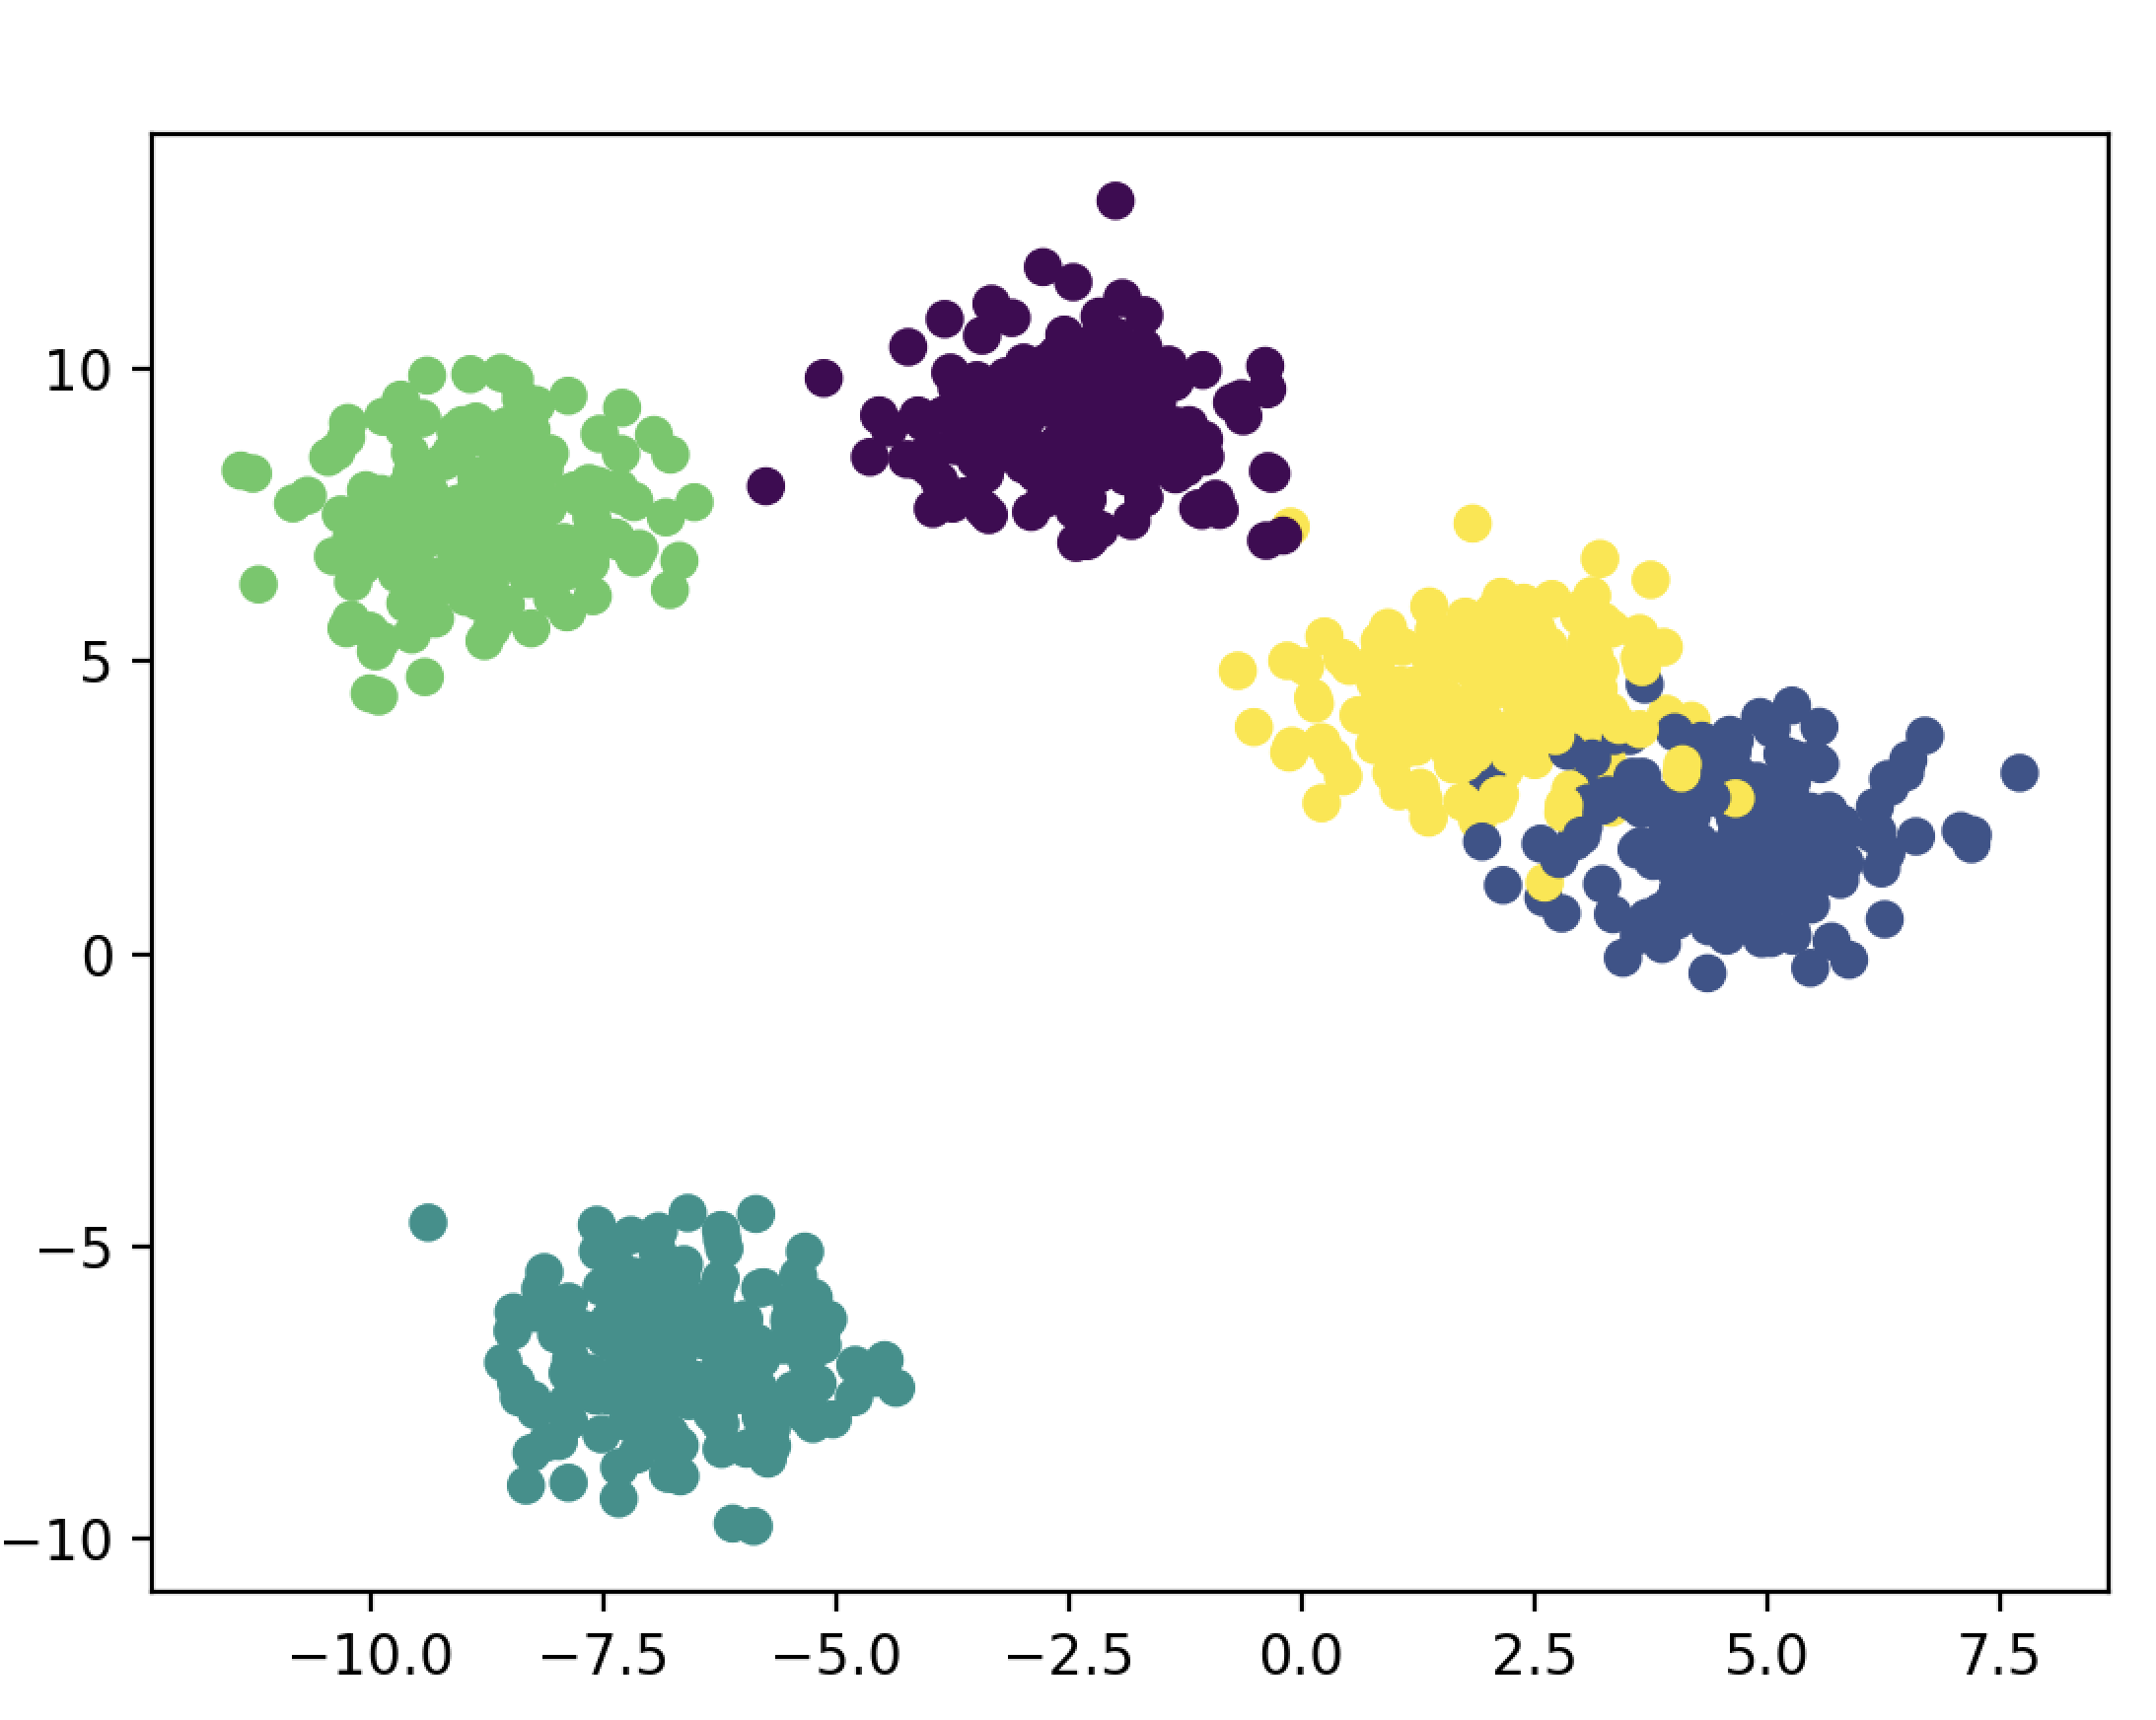
\includegraphics[width=0.8\linewidth]{images/blobs}
	\caption{Сгенерированный набор данных}
	\label{img:blobs}
\end{figure}

Алгоритм работы кода в \textit{code/main.py}:
\begin{enumerate}
	\item Создаётся по экзмпляру класса Perceptron и SGDClassifier;
	\item Считывается датасет из файла \textit{generated\_dataset.csv};
	\item Запускается обучение модели;
	\item Рисуется \textit{Decision surface};
	\item Рисуется набор данных;
	\item В консоль выводятся метрики, достигнутые на тестовой выборке.
\end{enumerate}

Следующие результаты были получены при инициализации класса перцептрона и линейного классификатора с дефолтными для библиотеки параметрами за исключением \textit{random\_state}=42, \textit{n\_jobs=}-1. Последний необходим для того, чтобы обучение использовало все доступные ядра CPU. Тестовая выборка составляет три десятых от всего набора данных. 

\begin{figure}[h]
	\centering
	\begin{subfigure}{0.49\linewidth}
		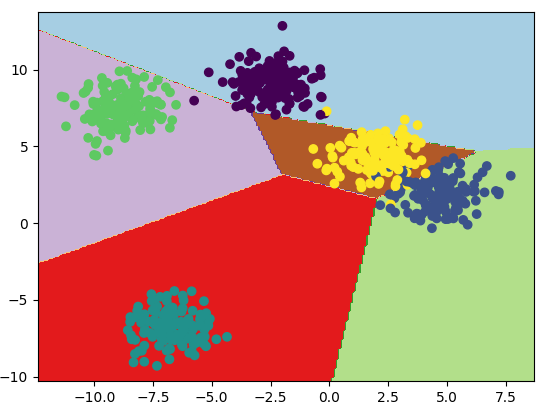
\includegraphics[width=\linewidth]{images/perceptron_train_blobs}
		\caption{Перцептрон: обучающая выборка}
	\end{subfigure}
	\begin{subfigure}{0.49\linewidth}
		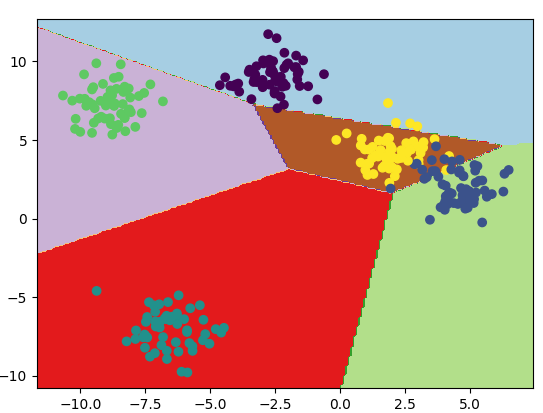
\includegraphics[width=\linewidth]{images/perceptron_test_blobs}
		\caption{Перцептрон: тестовая выборка}
	\end{subfigure}
	\begin{subfigure}{0.49\linewidth}
		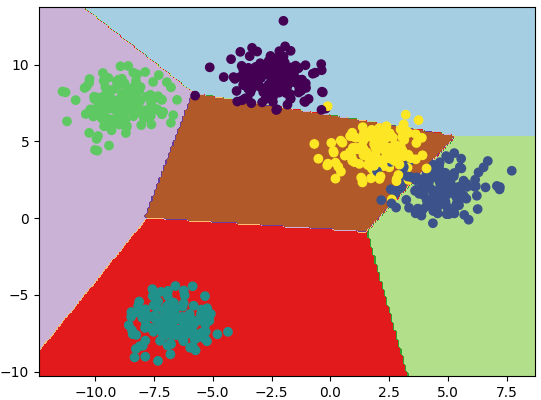
\includegraphics[width=\linewidth]{images/sgd_train_blobs}
		\caption{Линейный классификатор: обучающий набор}
	\end{subfigure}
	\begin{subfigure}{0.49\linewidth}
		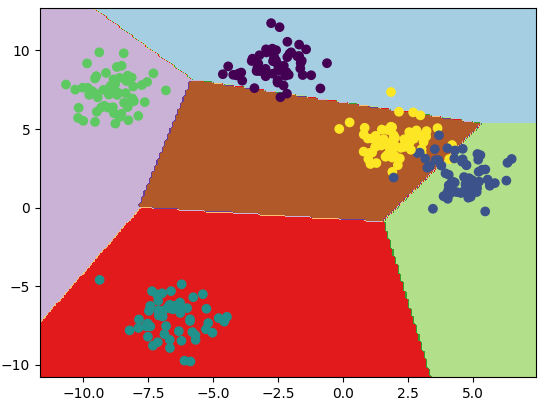
\includegraphics[width=\linewidth]{images/sgd_test_blobs}
		\caption{Линейный классификатор: тестовый набор}
	\end{subfigure}

	\caption{\textit{Decision surface} и выборки данных}
	\label{img:blobs}
\end{figure}

Метрики на тестовом множестве показаны в таблице \ref{tbl:first_blobs_metrics}.
\begin{table}[h]
	\centering
	\begin{tabular}{|c|c|c|c|c|}
		\hline
		& \textbf{accuracy} & \textbf{precision} & \textbf{recall} & \textbf{f1} \\\hline
		Perceptron    & 0.9433 & 0.9487 & 0.9458 & 0.9449 \\\hline
		SGDClassifier & 0.9500 & 0.9558 & 0.9520 & 0.9517 \\\hline
	\end{tabular}
	\caption{Метрики на тестовом множестве}
	\label{tbl:first_blobs_metrics}
\end{table}

Статистика и картинки получены следующим скриптом:\\
\noindent\fbox{%
	\parbox{\textwidth}{%
		\centering
	python3.8 code/main.py}%
}

Так как однослойный перцептрон в своей основе имеет тот же принцип, что и линейный классификатор, попробуем добиться одинаковых результатов на обеих моделях. 


\begin{table}[h]
	\centering
	\begin{tabular}{|c|c|c|c|c|}
		\hline
		& \textbf{accuracy} & \textbf{precision} & \textbf{recall} & \textbf{f1} \\\hline
		Perceptron    & 0.8167 & 0.8324 & 0.8229 & 0.8009 \\\hline
	\end{tabular}
	\caption{Перцептрону указана функция регуляризации \textit{$l_2$}}
\end{table}

Скрипт получения такого результата:

\noindent\fbox{%
	\parbox{\textwidth}{%
		\centering
	python3.8 code/main.py -{}-penalty\_perceptron l2}%
}

\begin{table}[h]
	\centering
	\begin{tabular}{|c|c|c|c|c|}
		\hline
		& \textbf{accuracy} & \textbf{precision} & \textbf{recall} & \textbf{f1} \\\hline
		Perceptron    & 0.9767 & 0.9774 & 0.9776 & 0.9774 \\\hline
	\end{tabular}
	\caption{Перцептрону добавлен флаг ранней остановки, если оценка на валидации перестаёт улучшаться}
\end{table}


Скрипт получения такого результата:

\noindent\fbox{%
	\parbox{\textwidth}{%
		\centering
	python3.8 code/main.py -{}-early\_stopping\_perceptron 1}%
}

Перцептрон с ранней остановкой перегнал по метрикам линейный классификатор из библиотеки \textbf{sklearn}. Попробуем улучшить его путём изменения входных параметров. Укажем флаг ранней остановки, который помог с перцептроном, и добавим знаки после запятой, чтобы лучше видеть картину при близости результатов:

\begin{table}[!h]
	\centering
	\begin{tabular}{|c|c|c|c|c|}
		\hline
		& \textbf{accuracy} & \textbf{precision} & \textbf{recall} & \textbf{f1} \\\hline
		Perceptron       & 0.9767 & 0.9774 & 0.9776 & 0.9774 \\\hline
		SGDClassifier    & 0.9667 & 0.9696 & 0.9682 & 0.9678 \\\hline
	\end{tabular}
	\caption{Линейному классификатору добавлен флаг ранней остановки. }
	\label{tbl:close_blobs}
\end{table}

Сейчас, судя по таблице \ref{tbl:close_blobs} разница по метрикам около одного процента.

Скрипт получения такого результата:

\noindent\fbox{%
	\parbox{\textwidth}{%
		\centering
	python3.8 code/main.py -{}-early\_stopping\_perceptron 1 -{}-early\_stopping\_sgd 1}%
}

\begin{table}[!h]
	\centering
	\begin{tabular}{|c|c|c|c|c|}
		\hline
		& \textbf{accuracy} & \textbf{precision} & \textbf{recall} & \textbf{f1} \\\hline
		Perceptron       & 0.9767 & 0.9767 & 0.9767 & 0.9767 \\\hline
		SGDClassifier    & 0.9700 & 0.9714 & 0.9713 & 0.9710 \\\hline
	\end{tabular}
	\caption{Линейному классификатору добавлен флаг ранней остановки и отключена функция регуляризации (по умолчанию включена и равна $l_2$).}
\end{table}

Это наименьшая разница в метриках, которую удалось добиться изменением параметров классов (без полного превращения линейного классификатора в перцептрон по параметрам). \textit{Decision surface} при этом получились следующие (рис. \ref{img:blobs_last}).

Скрипт получения такого результата:

\noindent\fbox{%
	\parbox{\textwidth}{%
		\centering
	python3.8 code/main.py -{}-early\_stopping\_perceptron 1 -{}-early\_stopping\_sgd 1 -{}-penalty\_sgd None}%
}

\begin{figure}[h]
	\centering
	\begin{subfigure}{0.49\linewidth}
		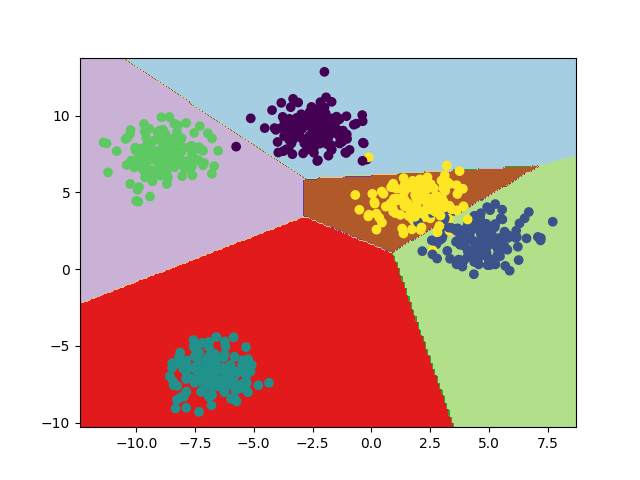
\includegraphics[width=\linewidth]{images/perceptron_train_blobs_last}
		\caption{Перцептрон: обучающая выборка}
	\end{subfigure}
	\begin{subfigure}{0.49\linewidth}
		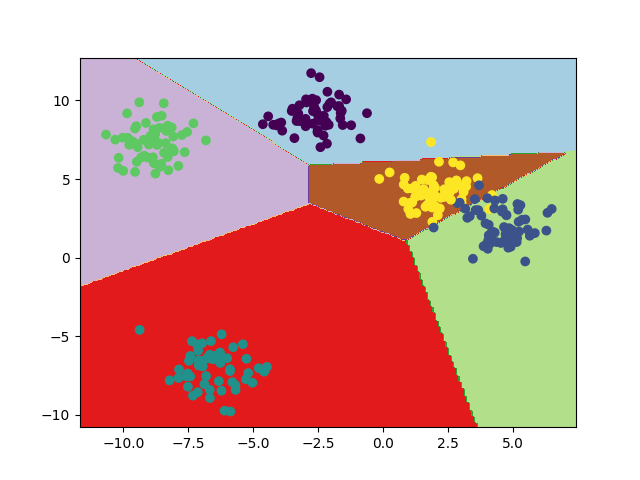
\includegraphics[width=\linewidth]{images/perceptron_test_blobs_last}
		\caption{Перцептрон: тестовая выборка}
	\end{subfigure}
	\begin{subfigure}{0.49\linewidth}
		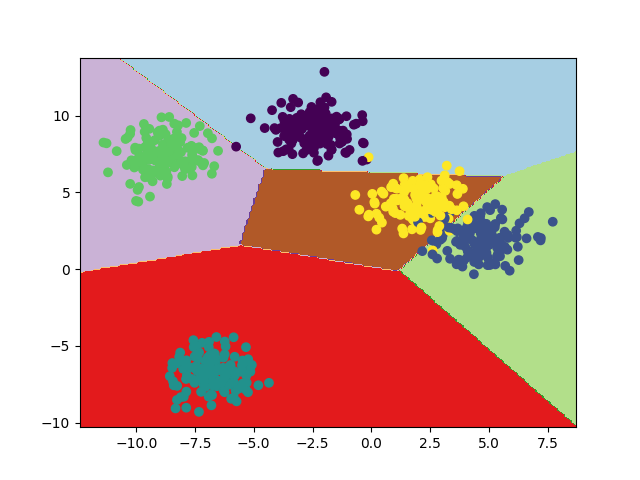
\includegraphics[width=\linewidth]{images/sgd_train_blobs_last}
		\caption{Линейный классификатор: обучающий набор}
	\end{subfigure}
	\begin{subfigure}{0.49\linewidth}
		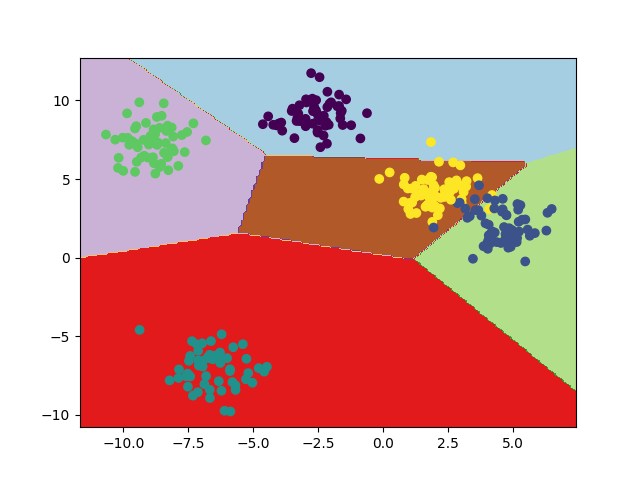
\includegraphics[width=\linewidth]{images/sgd_test_blobs_last}
		\caption{Линейный классификатор: тестовый набор}
	\end{subfigure}

	\caption{\textit{Decision surface} и выборки данных с новыми параметрами моделей}
	\label{img:blobs_last}
\end{figure}
\subsection{Авила датасет}
Набор данных был получен из 800 изображений Библии Авилы, сделанная в 12 веке копия Библии на латыни. Цель набора "--- подготовить модель для определения букв по шаблону, чтобы помогать переписывающему. Классами в наборе данных являются 11 букв: A, B, C, D, E, F, G, H, I, W, X, Y.

Характеристика датасета:
\begin{itemize}
	\item количество примеров "--- 20867;
	\item количество атрибутов "--- 10 (расстояние между колонками, верхний отступ, нижний отступ, использование, номер строки, модульное соотношение, интерлиньяж, вес, максимальное число, частное модульного соотношения и интерлиньяжа);
	\item проведена z-нормальзиация;
	\item пропущенных значений нет;
	\item несбалансирован;
	\item количество классов "--- 11.
\end{itemize}

Перед тем, как передавать датасет на обучение моделям, было проведено кодирование ответов: отсортированному множеству букв было присвоено число из натурального множества с нулём (A "--- 0, B "--- 1, \dots, Y "--- 11).


\begin{table}[!h]
	\centering
	\begin{tabular}{|c|c|c|c|c|}
		\hline
		& \textbf{accuracy} & \textbf{precision} & \textbf{recall} & \textbf{f1} \\\hline
		Perceptron       & 0.4496 & 0.2965 & 0.1992 & 0.2123 \\\hline
		SGDClassifier    & 0.5462 & 0.3718 & 0.3728 & 0.3480 \\\hline
	\end{tabular}
	\caption{<<Чистый>> запуск без параметров.}
\end{table}

\noindent\fbox{%
	\parbox{\textwidth}{%
		\centering
	python3.8 code/main.py -{}-enable\_generated\_dataset 0 -{}-enable\_archive\_dataset 1}%
}
\newline

Воспользовавшись \textbf{GridSearchCV}, были получены параметры, при которых перцептрон прибавляет в каждой метрике:

\begin{table}[!h]
	\centering
	\begin{tabular}{|c|c|c|c|c|}
		\hline
		& \textbf{accuracy} & \textbf{precision} & \textbf{recall} & \textbf{f1} \\\hline
		Perceptron       & 0.4870 & 0.3095 & 0.2626 & 0.2678 \\\hline
		SGDClassifier    & 0.5462 & 0.3718 & 0.3728 & 0.3480 \\\hline
	\end{tabular}
	\caption{Запуск перцептрона с параметрами, подобранными \textbf{GridSearchCV}.}
\end{table}

\noindent\fbox{%
	\parbox{\textwidth}{%
		\centering
	python3.8 code/main.py -{}-enable\_generated\_dataset 0 -{}-enable\_archive\_dataset 1 -{}-alpha 1 -{}-early\_stopping\_perceptron 1 -{}-eta0 0.1 -{}-tol 1 -{}-validation\_fraction 0.2}%
}\\

Попробуем зайти с другой стороны и изменим датасет. Оставим только те классы, количество примеров которых превышает тысячу: A(8572), E(2190), F(3923), H(1039), I(1663), X(1044). 

Получаем следующие метрики качества обучения (таблица \ref{tbl:squeezed_dataset}):
\begin{table}[!h]
	\centering
	\begin{tabular}{|c|c|c|c|c|}
		\hline
		& \textbf{accuracy} & \textbf{precision} & \textbf{recall} & \textbf{f1} \\\hline
		Perceptron       & 0.5401 & 0.5062 & 0.4778 & 0.4859 \\\hline
		SGDClassifier    & 0.6036 & 0.5821 & 0.4828 & 0.4986 \\\hline
	\end{tabular}
	\caption{Метрики с урезанным набором данных.}
	\label{tbl:squeezed_dataset}
\end{table}

Результат был достигнут следующим скриптом:

\noindent\fbox{%
	\parbox{\textwidth}{%
		\centering
	python3.8 code/main.py -{}-enable\_generated\_dataset 0 -{}-enable\_archive\_squeezed\_dataset 1}%
}\\

Наблюдаем, что каждая метрика улучшилась на несколько процентов. Урезанный набор данных более сбалансирован, чем исходный. Дальнейшее увеличение значений метрик осложнено двумя факторами:
\begin{itemize}
	\item невозможность закодировать ответы методом \textit{one hot encoding} "--- реализация \textbf{sklearn} не позволяет моделям принимать эталонные ответы в виде векторов с размерностью не равной 1;
	\item линейность моделей "--- линейная неразделимость классов не позволяет добиться точных моделей только с линейными <<разграничителями>> классов (гиперплоскость).
\end{itemize}
\end{document}